\documentclass[11pt]{article}
\usepackage{amsmath}
\usepackage{float}
\usepackage{graphicx}
\usepackage{caption}
\usepackage{mathabx}
\usepackage{subcaption}
\usepackage{algorithm}
\usepackage{algpseudocode}
\begin{document}

\section{Abstract}

\section{Introduction}
Poisson's equation is an elliptic partial differential equation of broad utility in theoretical physics. For example, the solution to Poisson's equation is the potential field caused by a given electric charge or mass density distribution; with the potential field known, one can then calculate electrostatic or gravitational (force) field. 

There are increasing number of method regarding solving this link of partial differential equation (PDE), such as finite difference method, finite element method and spectral method. 

In this project, we want to try MPI and OpenMP to solve Poisson equation
\begin{equation}
	\Delta u(\mathbf{x}) = f, \quad \mathbf{x} \in \Gamma
\end{equation}
in a irregular domain $\Gamma$ with Dirichlet boundary condition $u(\mathbf{x}) = g(\mathbf{x}), \mathbf{x}\in \partial\Gamma $ with finite element method.
  
\section{Results}
\subsection{One dimensional case}
\subsection{formula of finite element method}
Consider problem  
\begin{equation}
\label{equ:poisson_equation}
	u''(x) = f(x) \quad x\in (0,1)
\end{equation}
with boundary condition $u(x)=0$ at the boundary. We introduce a triangulation of the domain $\Omega = [0,1] $ into nonoverlapping elements:
\begin{equation}
\label{equ:triangulation}
	T_h = \{K_1,K_2,...\}
\end{equation}
such that $\Omega = \cup_{K\in T_h}K$. Now consider the space of continuous functions that are piecewise linear on the triangulation and zeros at the end points:
\begin{equation}
\label{equ:basis}
	V_h =\{v\in C^0([0,1]):v|_{K} \in \mathcal{P}_1(K) \forall K \in T_h, v(0) = v(1) = 0\}.
\end{equation}
Here $\mathcal{P}_p(K)$ is the space of polynomials on $K$ of degree at most $p$. Define a basis $\{\varphi_i\}$ for $V_h$ by the basis functions $\varphi_i\in V_h$ with $\varphi_i(x_j) = \delta_{ij}$, for $i,j = 1,...n$. The figure is shown in the following figure
\begin{figure}[htp]
\centering
	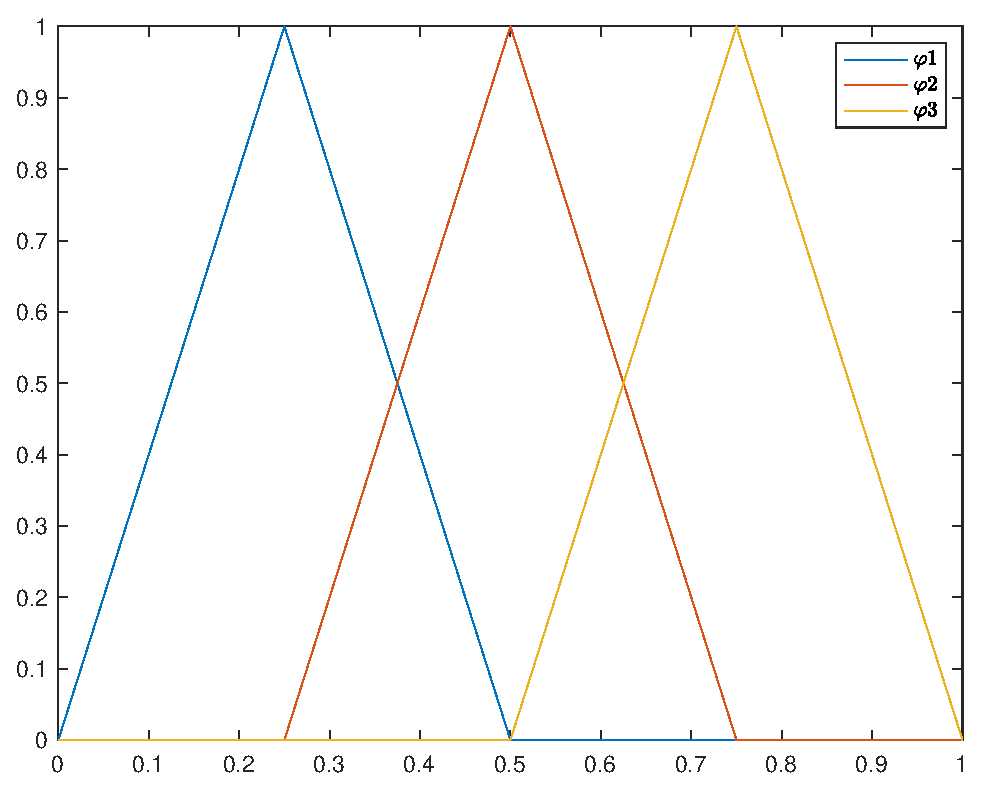
\includegraphics[width=0.5\textwidth]{basis_figure}
	\caption{what}
\end{figure}
Our approximate solution $u_h(x)$ can then be written in terms of its expansion coefficients and the basis functions as
\begin{equation}
\label{equ:appro}
	u_h(x) = \sum_{i = 1}^n u_i\varphi_i(x),
\end{equation} 
where we note that this particular basis has the convenient property that $u_h(x_j) = u_j$, for j = 1,...n.

A Galerkin formulation can be stated as: Find $u_h \in V_h$ such that
\begin{equation}\label{equ:formula}
	\int_0^1u_h'(x)v'(x) = \int_0^1f(x)v(x) dx, \quad \forall v \in V_h 
\end{equation}
In particular, \eqref{equ:formula} should be satisfied for $v = \varphi_i$ , $i = 1,...,n$, which leads to $n$ equations of the form
\begin{equation}
	\int_0^1 u_h'(x)\varphi_i(x)dx = \int_0^1\varphi_i(x)f(x)dx, \quad i = 1,...,n
\end{equation}
Insert the expression \eqref{equ:appro} for the approximate solution and its derivative, $u_h'(x) = \sum_{i=1}^n u_i\varphi'_i(x)$.
Change the order of interation:
\begin{equation}
	\sum_i^n u_j\left[\int_0^1\varphi_i'(x) \varphi_j'(x)\right]= \int_0^1\varphi_i(x) dx, \quad i = 1,...,n
\end{equation}
This is a linear system of equations $A\mathbf{u} = \mathbf{f}$, with $A = [a_{ij}]$, $\mathbf{u} = [u_i]$, $\mathbf{f} = [f_i]$, for $i,j = 1,...,n$, where
\begin{align}
	a_{ij} = \int_0^1\varphi'_i(x)\varphi'_j(x)dx \\
	f_i  = \int_0^1f(x)\varphi_i(x) dx
\end{align}

\subsection{Parallel computation strategy}
First we try Gauss Seidel method to solve the linear system defined in the formal section. The brief introduction of the Gauss Seidel method is shown belew
\begin{algorithm}
\caption{Gauss seidel method}\label{alg:gauss_seidel}
\begin{algorithmic}
\Require $A = (a_{ij})$,$f = f_i$
\State $\epsilon=1$
\While{$\epsilon \leq 1e-3$}
\State \textbf{for} $i$ \textbf{from} $1$ \textbf{until} $n$ \textbf{do}
\State \quad $\sigma \leftarrow 0$
\State \quad \textbf{for} $j$ \textbf{from} $1$ \textbf{until} $n$ \textbf{do}
\State \quad \quad \textbf{if} $j \neq i$
\textbf{then}
\State \quad  \quad  $\sigma$ $\leftarrow \sigma + a_{ij}u_j$
\State \quad  \quad \textbf{end if}
\State \quad \textbf{end} ($j$ - loop)
\State $u_i \leftarrow \frac{1}{a_{ii}} (f_i - \sigma)$
\EndWhile
\end{algorithmic}
\end{algorithm}
The advantage of the Gauss Seidel method is that it's easy to parall computing. The $u_i$ can be updated independently because they only need the information of the last step. We try to use Openmp and MPI to parallel compute the result.  
The numerical result is shown in the Figure
\begin{figure}
    \centering
    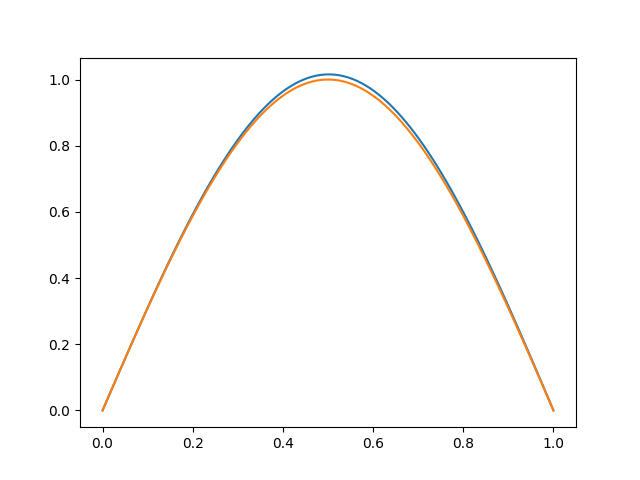
\includegraphics[width = 0.5\linewidth]{../CPP_code/1D_problem/openmp_version_gauss_seidel/result.png}
    \caption{The comparison result of the exact result and the numerical result, when the domain is decomposed into 10 equal part.}
    \label{fig:result comparison}
\end{figure}

\section{Discussion}

\end{document}
